\section{Introducción a C++}

\subsection{El lenguaje C++}

\begin{frame}[t]{C++}
\begin{columns}[T]

\column{.5\textwidth}

\begin{itemize}
  \item Un lenguaje de \textmark{programación de sistemas}:
    \begin{itemize}
      \item Abstracciones ligeras.
      \item Genera código binario.
      \item Altamente eficiente.
      \item Utilizado en muchos dominios.
    \end{itemize}

  \mode<presentation>{\vfill\pause}
  \item Diversos \textmark{estilos} soportados:
    \begin{itemize}
      \item Abstracciones de datos.
      \item Programación orientada a objetos.
      \item Programación genérica.
      \item Programación funcional.
      \item Programación asíncrona.
      \item Concurrencia.
    \end{itemize}
\end{itemize}

\column[T]{.5\textwidth}

\pause
\vspace{-1em}
\begin{center}
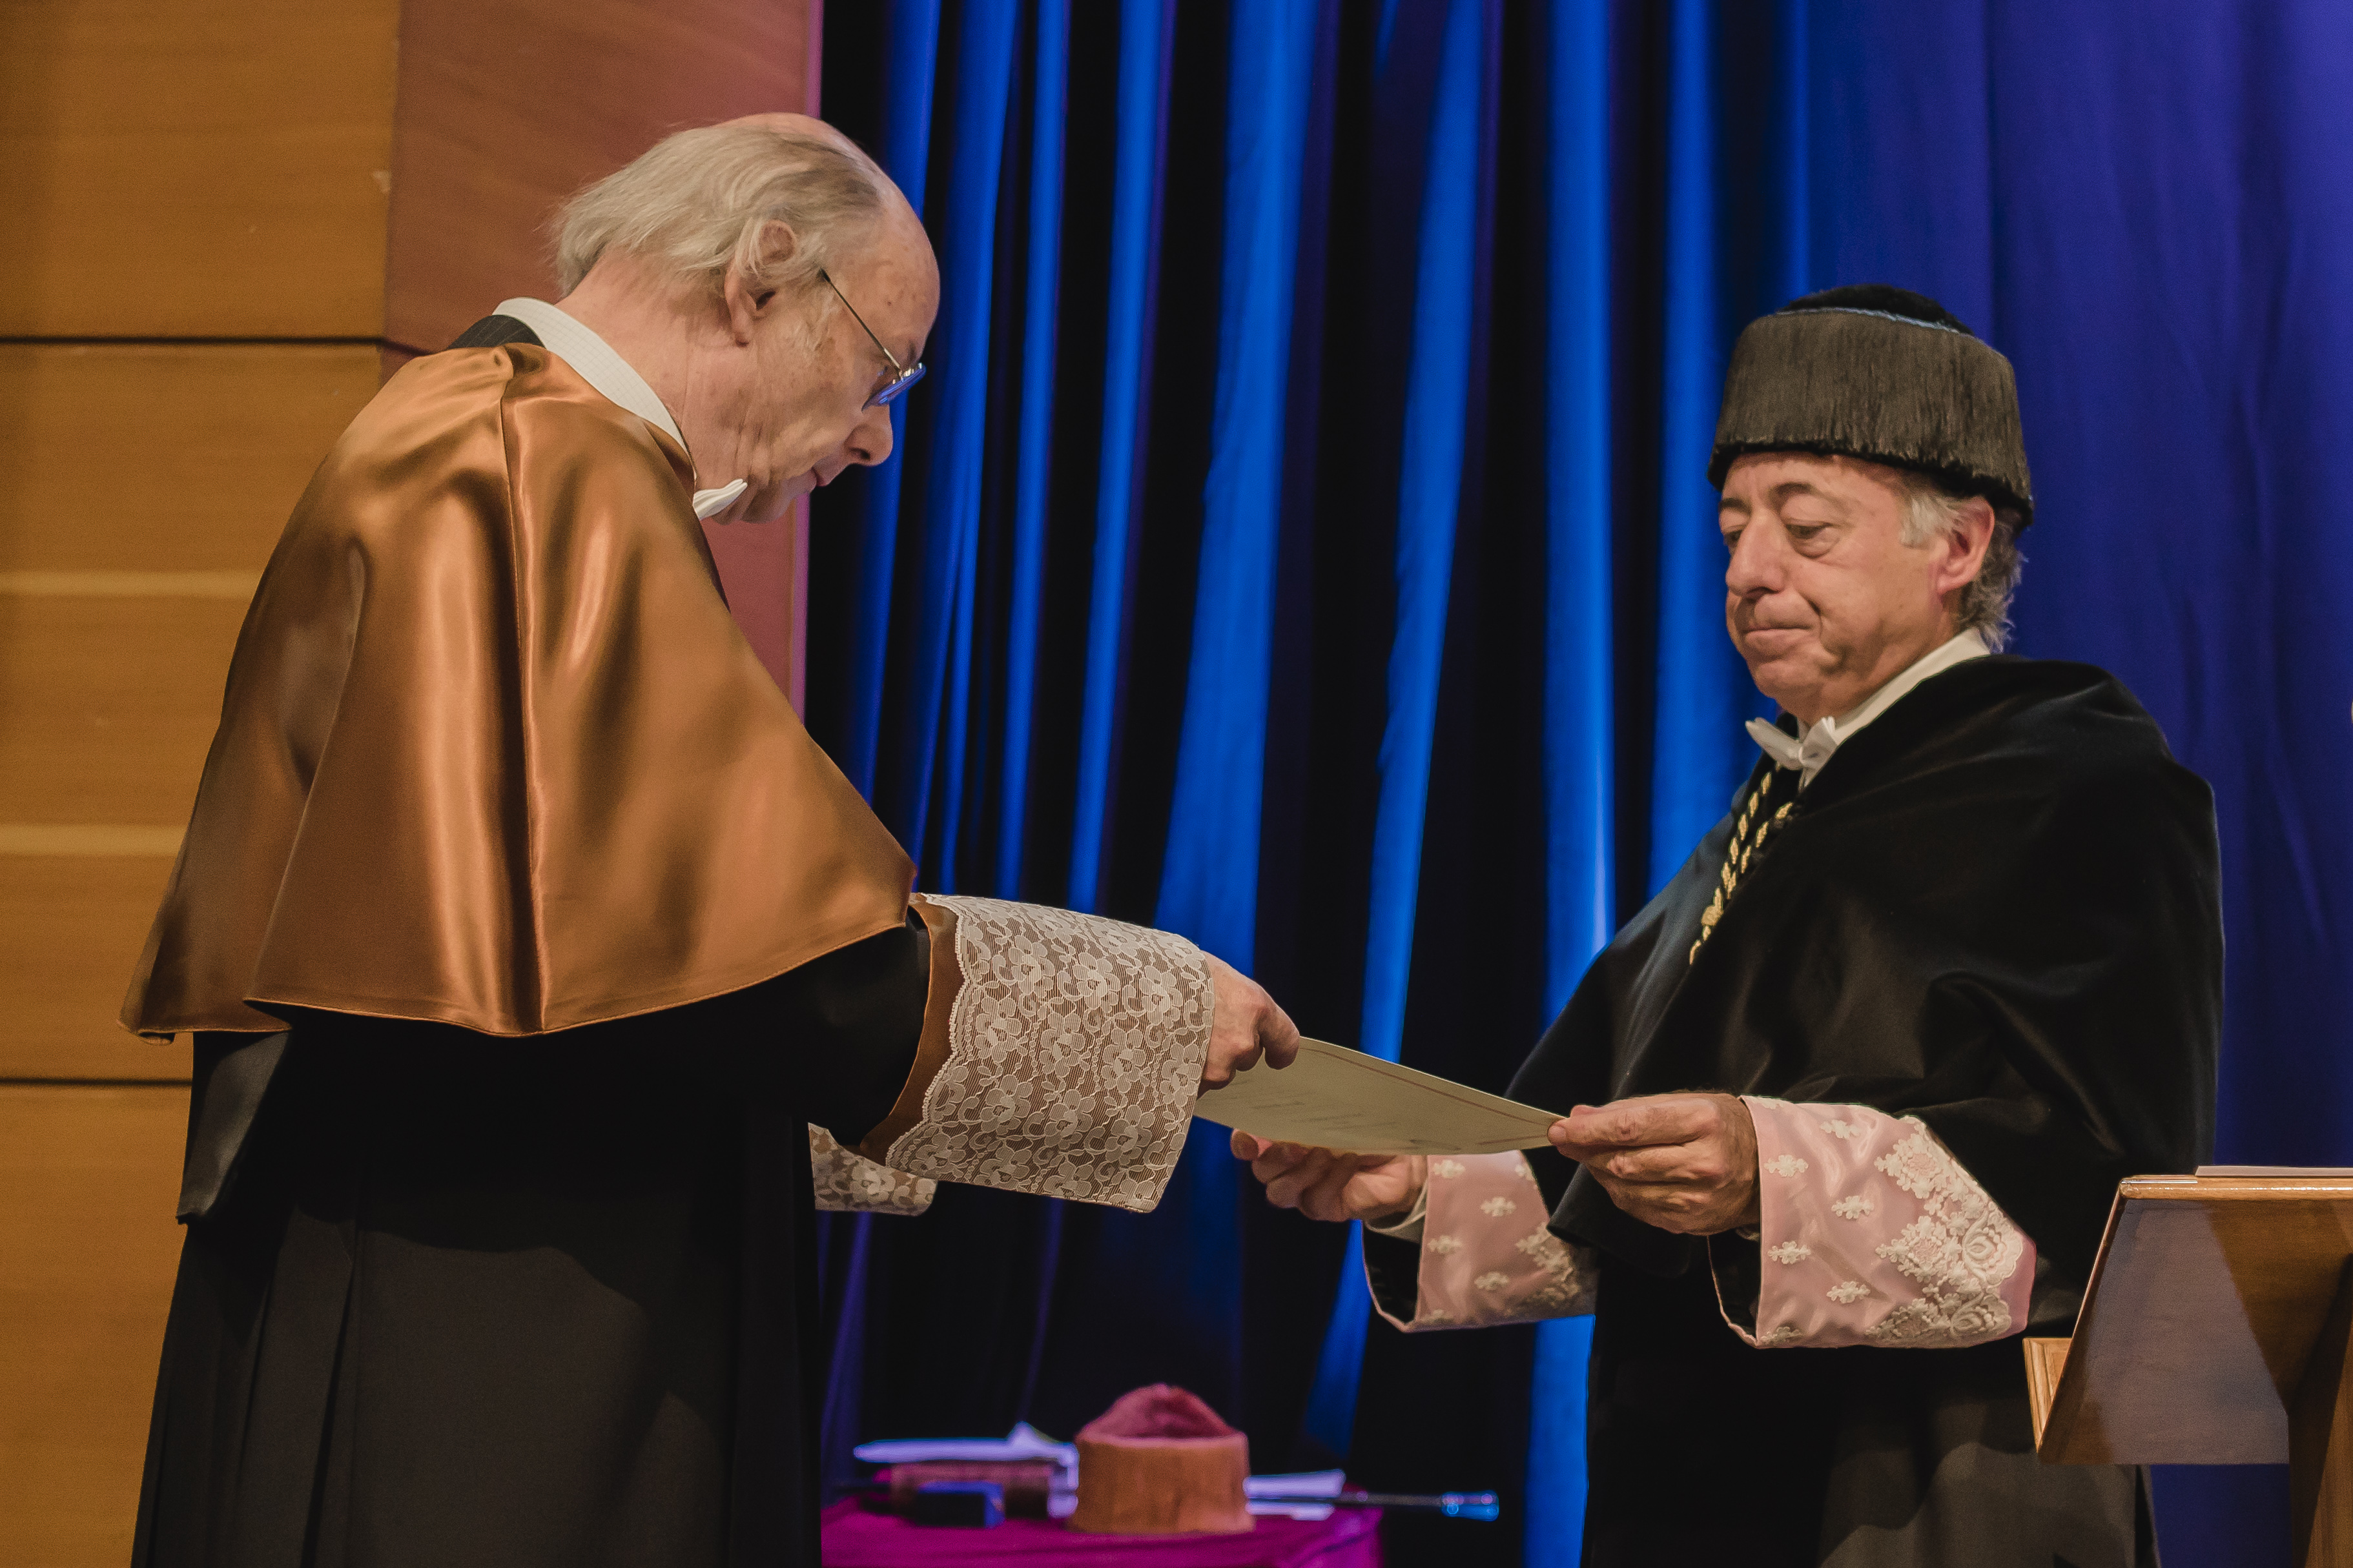
\includegraphics[width=.5\textwidth]{images/bjarne-honoris.jpg}
\end{center}

\begin{itemize}
  \item Diseñado por \textgood{Bjarne Stroustrup}.
\end{itemize}

\pause

\includegraphics[width=.5\textwidth]{images/logo-iso.png}

\includegraphics[width=.2\textwidth]{images/logo-cpp.png}

\begin{itemize}
  \item Serie ISO/IEC 14882.
\end{itemize}


\end{columns}
\end{frame}
